\documentclass{article}
\usepackage[utf8]{inputenc}
\usepackage[english]{babel}
\usepackage[colorinlistoftodos]{todonotes}

\title{MAS report}
\author{Emma Machielse, Federico Tavella, Alessandro Tezza}
\date{\today}

\begin{document}

\maketitle Final Report MAS

\todo[inline]{max 10 pages. \textbf{readability}; grammar, syntax, scientific style, reference fig and tables.\textbf{ completeness}; what is done, why and the results, motivation design choice, how does system work}

\section{Introduction}
Public transport is an universal subject of traveller complaints, targeted at the waiting and travel time. Attempts of transportation companies to reduce costs often have a detrimental effect on travelling time. A network of intelligent autonomous transportation units could optimize for lowering costs and travelling time. To illustrate this a multi-agent system is created for intelligent bus transport in Amsterdam. The goal of this system is to transfer passengers as efficient as possible. Several methods stated in game theory \cite{intromultiagentsystems} are implemented to create this system
, like communication between buses, coordination and negotiation. 

\section{Framework}
We chose to organise our system according to the Belief-Desire-Intention architecture \cite{caillou2017simple}. Intentions are future directed and trigger certain actions \cite{multiagentsystems}. This framework facilitates flexibility in generating actions, because an agent can switch between intentions depending on the state of the environment. 
\newline
A desire is unconstrained and is what implies the intentions \cite{multiagentsystems}. In the transportation system the desire for all buses is to transport passengers. The beliefs contain the knowledge the bus needs to fulfill the desire. This comes down to the route along which a bus can travel. More flexible knowledge that the buses have are contained in local variables. 
\newline 
The desire implies several intentions that generate actions to bring transportation into practice. Intentions are updated and changed, when the secondary actions are completed or when the scenario changes. 
\newline
The buses are self-interested, which means they have their own beliefs and intentions \cite{multiagentsystems}. This can lead to agreeable or conflicting goals, which is the foundation for social interaction. This interaction takes place through communication. The communication between buses is based on the FIPA ontology \cite{fipa}. The communication message contains several parameters; the id of the sender, the id of the receiver, the content and a performative. A performative can be described as the message goal, which can basically be either to inform or to request. 

\section{Conceptual description and strategy}
This section explains the various agent concepts used, how they are designed and implemented, and along which strategies. Four types of costs shape our strategies, the amount of money spend, the average waiting time, the amount of messages send, and the amount of people waiting. Costs arise by travelling and buying more buses. To reduce costs, the buses need to transport travellers efficiently. The more passengers they can transport in the shortest amount of time, the lower the costs will be.

\subsection{transportation and coordination}
Buses are allowed to travel according to a specific route. This route describes the connections between 24 bus stops. A number of alterations have been done to the route in order to increase transportation efficiency. 
\paragraph{different fixed schedules}
In order to reduce the amount of time a passenger spends in a bus, the schedule is split into four different areas. They can be classified under the labels "West", "North", "Center" and "East". Splitting the route has two advantageous effects. A bus has to complete a shorter distance before passing the same stop again, so waiting time will be reduced. The time that a traveller spends in the bus will be shorter, which will reduce chances of buses being full and unable to pick up other travellers.
\newline
This solution does occasionally require transferring passengers from one area to another. This reduces the advantageous effects. Transfer passengers will have to wait at two bus stops before reaching their destination. To enable transportation of people between bus stops in different schedules, a transfer station is assigned. Stop 3 (\texttt{Centraal}), is a shared stop for all four schedules. If a bus picks up a passenger with a destination that is not in its schedule, it drops the passenger off at the shared stop. At the shared stop, buses only pick up passengers with a destination that is in their schedule. 
\paragraph{Direction-based pick up}
Another alteration to the route, is the implementation of a bidirectional transportation in each area. This will ensure that passengers won't be picked up by a bus,  that needs to complete a large distance before reaching their destination. This increases transportation efficiency, since buses carry passengers for a shorter amount of time and are thus able to carry more passengers. 
\newline
Each bus picks up only the passengers whose destination is closer in its schedule compared to the reverse one. If this is not the case, the passengers are waiting for a bus moving in the opposite direction. Thus travelling time of passengers is reduced. 
\newline
The number of buses assigned to either direction is evenly distributed. This ensures that travellers do not have to wait too long, before a bus in their direction arrives for pick-up. Buses created with an odd ID are moving along the \textit{reverse version} of the schedule for their area.

\subsection{Roles}
To ensure that the buses cooperate efficiently, they are assigned specific roles. Roles differ in their ancillary responsibilities and so a hierarchy of buses was created. 
\newline
Roles can also define the \textit{behaviour} of a bus. Using roles makes it easy to change the behaviour of a bus. 
\paragraph{Roles of responsibility}
A major responsibility is buying new buses, in case of shortage. If all buses would be able to, this would happen inefficiently and increase costs unnecessarily. Therefore only the first created bus with \texttt{ID = 24} is assigned this responsibility. This bus is on top of the hierarchy, and its role is defined as \textit{global coordinator}. Its second responsibility is assigning roles to other buses.
\newline
The \textit{global coordinator} adds buses based on shortage. Shortage is defined as the difference between the total number of people waiting, and the total bus fleet capacity. The cheapest bus type that is able to manage the amount of waiting people, is added.
\newline
\todo[inline]{I think this type of buss adding rule changed??}
One step down in the hierarchy, are the \textit{local coordinators}. They are each responsible for one of the four areas in Amsterdam. The \textit{global coordinator} is assigned to the "Centre", the buses with \texttt{ID = 25, 26 and 27} are responsible for "West", "East" and "North" in that order. The coordinators keep track of their area, by listing the buses assigned to their area, their fleet capacity and the number of people waiting. They ask other coordinators for buses if they have a shortage in their area, or they request for newly added buses. 
\newline
\paragraph{Roles for behaviour}
The roles that can be assigned to the other buses through communication are \textit{scout} and \textit{simple}. These roles define the travelling behaviour of a bus. \textit{Simple} buses stop moving when they are empty and they reach an empty bus stop. This reduces travelling costs for a scenario in which the few people waiting, can be managed by other buses. A similar behavioural condition goes for all the buses. For the extreme scenario in which the total amount of people waiting is zero, none of the buses move. 
\newline
A scout is always moving and is not allowed to stop and wait.This ensures that some buses are continuously travelling. Even when the amount of passengers waiting is low, the few people left waiting will still be picked up.

\subsection{Communication}
As stated before, to enable social interaction between agents with conflicting or agreeable goals, a form of communication is implemented. This communication happens through the exchange of messages. A bus sends a message with a specific goal, and the receiver performs actions based on the content.
\paragraph{Ontology}
To take into account the possibility of messages with different purpose, we defined the following ontology for communication: \texttt{"message\_type content"}. Where  \texttt{message\_type} is the header of the message, or the performative \cite{fipa}. This is a string that described the goal of the message. Then \texttt{content} contains the effective content of the message. For example, if we want to promote a bus to the role \textit{scout}, the message would be in the form \texttt{"promotion scout"}. We implemented this ontology, so that buses know how what to use the content of the message for, based on the performative. The perfomatives of the messages can be promoting, assigning, requesting help, offering help, accepting help, requesting a bid, bidding and reallocating. 
\newline
The reception of the messages goes as following. At every tick a bus checks its incoming messages. It can retrieve the new messages from the inbox history. To check whether a message is new, its tick is compared to the last tick at which the agent checked its inbox. This last tick is represented by a \textit{locally stored variable}. The performative of the message, implies how to interpret the content. Based on the content the bus changes intentions and/or performs certain actions.

\subsection{Promoting}
Communication is used in order to enable the \textit{global coordinator} to promote and demote buses to different roles. In a critical scenario, all buses are promoted to scout, to ensure that no bus will stop travelling. The situation is defined as critical when more than 1000 people are waiting. This number is a parameter, which is tuned to attempt an optimal value.
\todo[inline]{Which amount is chosen?? I put 1000 there randomly}
Once the danger situation has been managed, the \textit{global coordinator} will demote the buses to a \textit{simple} role again. Consequently, they are allowed to stop and wait to reduce travelling costs.

\subsection{Group decisions}
The division of the route into four areas can lead to certain scenarios that involve unnecessary costs. Steps are taken to deal with a situation, where one area has a shortage of buses whereas the other area has a remnant. 
\newline
Local coordinators keep track of all the buses that move in their area. In addition, they compare the amount of people waiting in their area with the fleet capacity. Based on this comparison, they decide whether they need more buses. If this is the case, they collaborate with the other coordinators. 
\newline
This collaboration is done by sending a message to the other coordinators. The message has performative \textit{request help} and the content is a number; the shortage of fleet capacity. The other coordinators check if they have remnant buses, and if so send a message with performative \textit{offer help} and the content is the id of the bus that is remnant. Upon receiving this offer, the coordinator adds this bus to its bus fleet. A reply is send with performative \textit{accept help} and again as content the id of the offered bus. The other coordinator removes the bus from its bus fleet. The offered bus receives a message with performative \textit{reallocate} and the content contains the bus id of its new coordinator. Based on this new coordinator, the bus retrieves its new schedule. As soon as it reaches the transfer stop, it changes area. In this way, local coordinators from different areas can exchange buses between them. Thus, buses are distributed more efficiently and costs associated to the creation of new buses are reduced.

\subsection{Negotiation}
When the \textit{global coordinator} adds a new bus based on a shortage of fleet capacity, it has assign the new bus to one of the four areas. The new buses should be used as efficiently as possible. Therefore it has to be decided which area the bus will be most useful to. To help the \textit{global coordinator} decide, a bidding system is implemented. 
\newline
After creating a a new bus, the \textit{global coordinator} sends a message to the \textit{local coordinators} of performative \textit{bid-request} and the content is the bus id of the newly added bus. The \textit{local coordinators} check their shortage; the difference between their fleet capacity and the number of people waiting in their area. They communicate \textit{bidding} and the shortage as content, to the \textit{global coordinator}. The coordinator with the highest bid is in most need of a new bus. The new bus is assigned to that coordinators area. The new bus receives a reallocation message.

\section{Refactored code}
For clarity and readability, the code is refactored. The agents.nls file is splitted into 5 files. The agents.nls code describes the core BSI framework, linked to action execution. Then there is an init file, that states how the first buses are created and initialised. The execute-intentions file describes the action functions needed for each intention. The messages file incorporates some utility functions to work with the messages. Finally we have a utils file that contains all the functions needed by the rest of the application. 

\section{Performance}
\todo[inline]{Whatevers done to increase performance by parameter tuning, for example parameter for promoting }
See table 1.
See figure \ref{fig:expense}
see figure \ref{fig:messages}
See figure \ref{fig:pass_waiting}
See figure \ref{fig:avg_tt}

\begin{figure}
\centering
\begin{minipage}{.5\textwidth}
  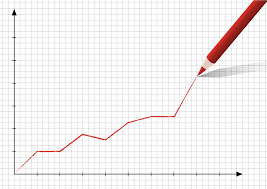
\includegraphics[width=.4\textwidth]{expenses.jpg}
  \caption{\label{fig:expense}Figure that displays the expenses of the buses.}
\end{minipage}%
\begin{minipage}{.5\textwidth}
  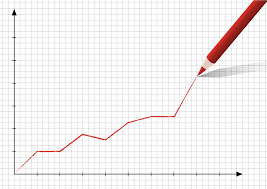
\includegraphics[width=.4\textwidth]{nr_messages.jpg}
  \caption{\label{fig:messages}Figure that displays the number of exchanged messages.}
\end{minipage}
\end{figure}

\begin{figure}
\centering
\begin{minipage}{.5\textwidth}
  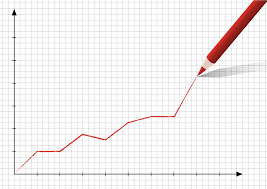
\includegraphics[width=.4\linewidth]{nr_pass_waiting.jpg}
  \caption{\label{fig:pass_waiting}Figure that displays the number of passengers waiting.}
\end{minipage}%
\begin{minipage}{.5\textwidth}
  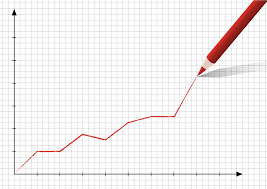
\includegraphics[width=.4\linewidth]{avg_tt.jpg}
  \caption{\label{fig:avg_tt}Figure that displays the average travelling time.}
\end{minipage}
\end{figure}

\section{Performance on test data}

See Table 1.

\begin{table*}
\begin{tabular}{ |c|c|c|c|  }
 \hline
 \multicolumn{4}{|l|}{Table 1. Performance results} \\
 \hline
  Measurement & Data set 1 & Data set 2 & Data set 3 \\
 \hline
  Avg travel time & 0 & 0 & 0\\
  Buses' expenses & 0 & 0 & 0\\
  Messages sent & 0 & 0 & 0\\
  Final amount waiting & 0 & 0 & 0\\
  Avg travel time remaining & 0 & 0 & 0\\
  Final avg travel time & 0 & 0 & 0\\
 \hline
\end{tabular}
\end{table*}

\subsection{Conclusion}
From the results can be concluded that...

\section{Discussion}
Some implementations that could have led to better performance of the system are the following.
\newline
The amount of occupied spots in each bus is local information, that can only be made known to other buses through communication. This information could have been used to make a more accurate estimation of the amount of buses needed for the travellers. Since the current system is very sensitive to adding new buses, the information did not seem valuable. To reduce the amount of messages send, this information is not communicated.

\newpage
\onecolumn
\bibliographystyle{ieeetr}
\bibliography{bib}

\end{document}
